%!TEX program = xelatex
% 完整编译方法 1 pdflatex -> bibtex -> pdflatex -> pdflatex
% 完整编译方法 2: xelatex -> bibtex -> xelatex -> xelatex
\documentclass[lang=cn,11pt]{elegantpaper}
\usepackage{listings}
\usepackage{fontspec}
\setmonofont{Consolas}

\title{南开大学教师信息Web检索系统}
\author{\href{https://github.com/Jack-Lio}{李伟}}

\institute{1711350   计算机科学与技术一班}

% 不需要版本信息,直接注释即可
%\version{0.07}
% 不需要时间信息的话,需要把 \today 删除。
\date{\today}


% 如果想修改参考文献样式,请把这行注释掉
\usepackage[authoryear]{gbt7714}  % 国标

\begin{document}

\maketitle

\begin{abstract}
\noindent 搜索引擎是我们经常使用的工具,能够大大方便我们对于信息的获取和知识的学习,在生活中搜索引擎的便捷性让我们只需要面对一个搜索框就能实现海量信息的检索,通过学习信息检索这门课程之后,对于其背后的实现机制有了基本的了解,在本次实验中,我基于对于课上所学习的检索系统相关知识和pagerank链接分析的理解,基于百度搜索引擎的样式实现一个对南开部分教师的web搜索系统,系统能够很好的支持网页爬取、链接分析、以及便捷的查询服务功能,此外,实现了较好的用户界面和交互机制,支持的查询服务包括短语查询、前缀查询、正则表达式查询、关系表达式形式的查询等;同时支持网页快照和网页跳转,并对查询所得到的的词项进行高亮处理和碎片化显示以及教师照片的显示,实现了非常友好的用户界面。
\keywords{网页爬取,Web搜索引擎,链接分析,web查询服务实现}
\end{abstract}


\section{实验要求与问题阐述}

\begin{figure}[htbp]
	\centering
	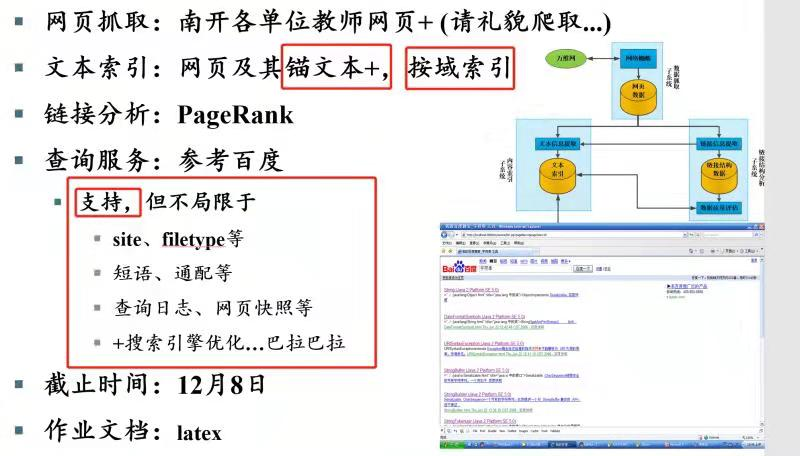
\includegraphics[width=0.6\textwidth]{0}
	\caption{作业要求 \label{fig:0}}
\end{figure}

如\figref{fig:0}所示,本次实验要求对南开大学各单位的教师介绍主页进行爬取,获取网页内容,实现简单的搜索引擎功能,能够进行查询反馈响应的网页链接,具体的相关要求如下:

\begin{itemize}
	\item 网页抓取:要求抓取南开各单位的教师网页
	\item 文本索引:要求对网页及其锚文本,以及相关的信息域进行索引构建
	\item 链接分析:要求对爬取的链接进行分析,帮助进行网页链接搜索的优化
	\item 查询服务:要求实现诸如site、filetype、短语或通配查询、查询日志记录、网页快照等工作
	\item 实现文档:要求编写实现文档
\end{itemize}



针对此次作业要求,可以了解到实验的重点问题在于网页数据的获取以及索引构建和查询服务实现,网页爬取需要基本的爬虫知识,索引构建允许使用第三方工具包支持,在这里可以使用Whoosh工具包,查询服务的实现可以参考主流的搜素引擎工具,如百度、google等,因此可以基本从这三个方面开展此次实验中的系统构建工作。

\section{实验环境}

\begin{itemize}
	\item 开发语言:python, html, javascript, css
	\item 开发平台:pycharm
	\item 主要工具包使用:numpy, whoosh, flask,scrapy
	\item 前端界面实现参考:百度搜索引擎
	\item 系统环境:window 10 专业版
	\item web后端环境:flask (启动时通过运行query.py文件启动后台flask进程)
\end{itemize}

\section{实现思路}
首先,本次实验主要分为三个步骤实现,分别是数据爬取,索引构建,查询服务实现,以下主要从这三个方面介绍本次实验的实现思路。

\subsection{数据爬取}
从南开大学官网的学院信息网页可以找到通往各个学院的链接,通过这个链接可以进入不同的学院进行进一步的数据爬取,南开大学的学院信息网页如\figref{fig:1}所示:


\begin{figure}[htbp]
	\centering
	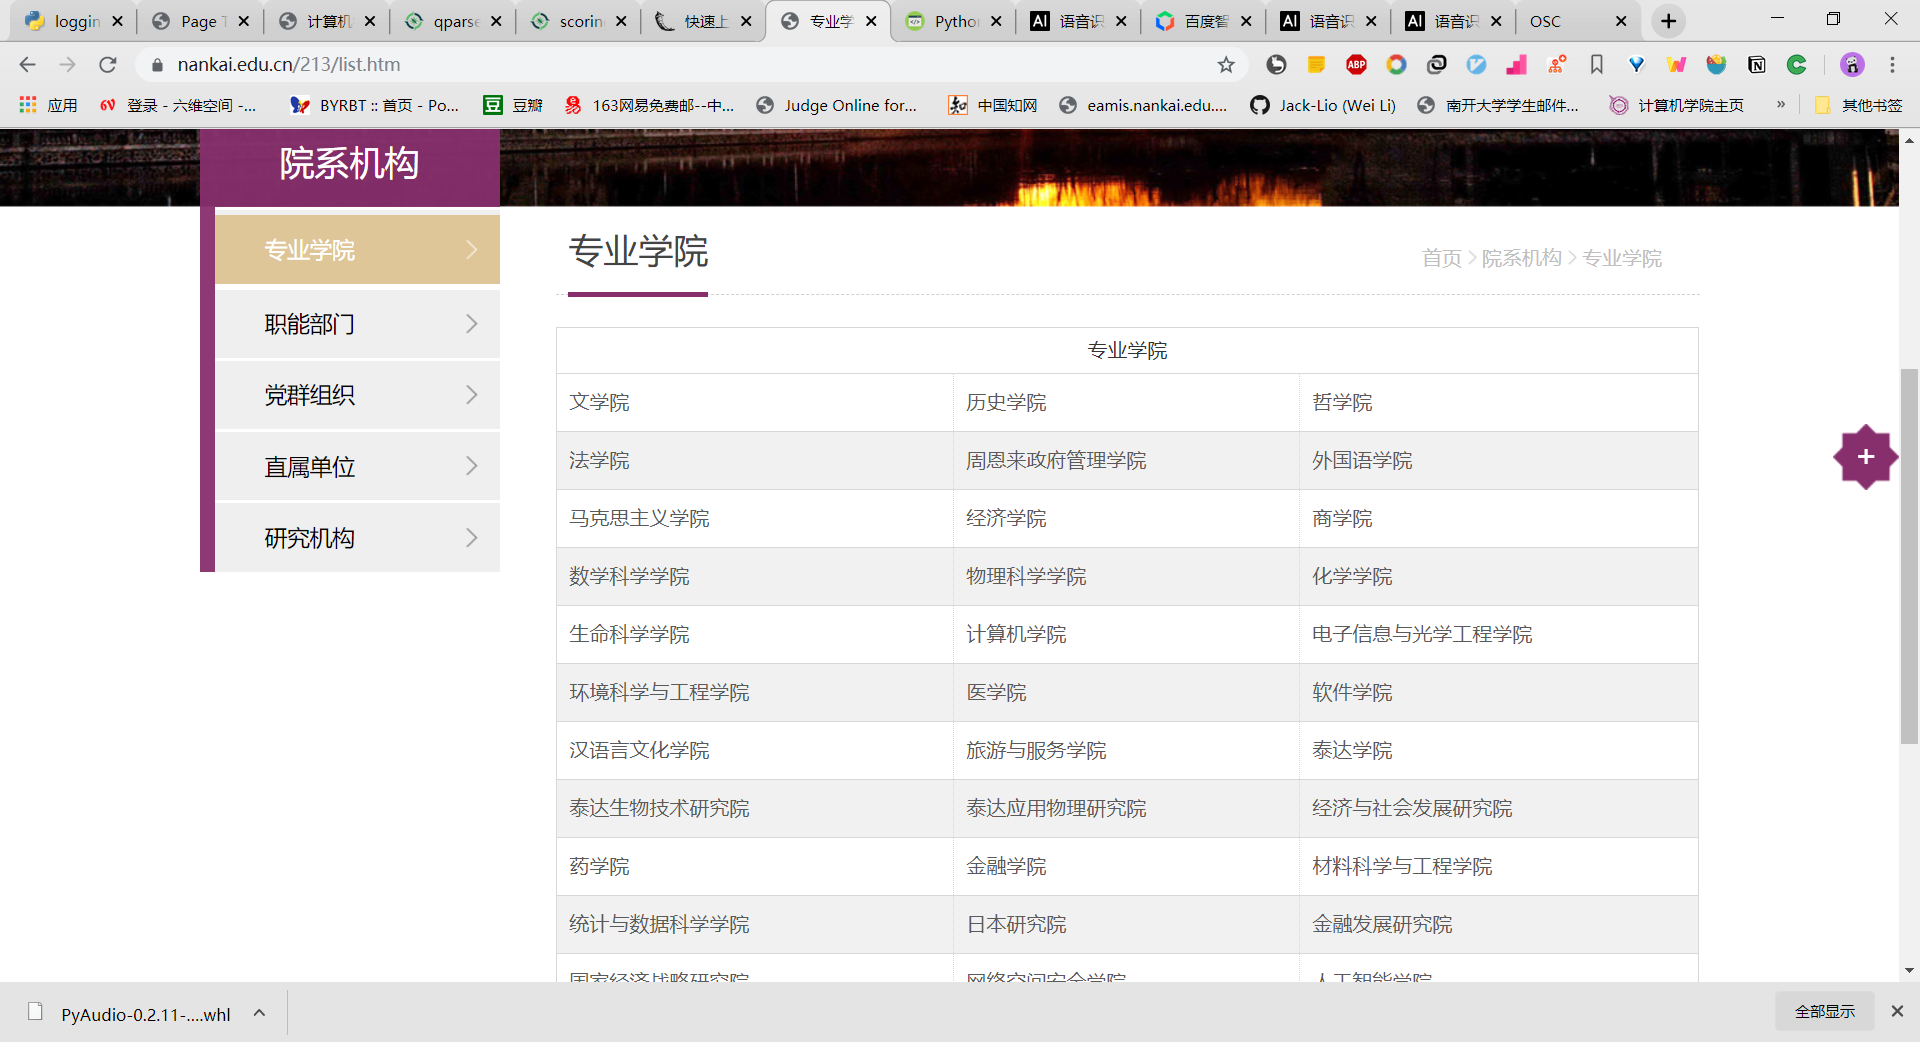
\includegraphics[width=0.6\textwidth]{1}
	\caption{南开大学各学院链接网页 \label{fig:1}}
\end{figure}

通过查看各个学院的网页的具体情况发现,由于不同学院的网站建站方式的不同,以及学院教师信息展示的不同,导致很难实现用统一的爬虫进行爬取,所以在本实验中我采用了为不同的学院编写不同的爬虫程序进行数据的爬取,爬取的数据主要包括网页的全部HTML代码(实现网页快照使用)、锚文本、教师照片、网页的主体内容。爬取的工具是利用了scrapy框架进行辅助爬取,之所以选择scrapy框架的原因在于其较简单的操作性以及较快速的爬取效率,能够减少爬虫的复杂度,降低难度。

\subsection{索引构建}

索引的构建是检索系统能够高效工作的核心,需要构建一个强大的索引才能够实现更多的功能,本次实验中的索引构建基于Whoosh全文检索的工具包,其提供了较为简单的索引构建流程以及提供了很多的查询服务接口,为之后的查询服务实现提供了很多的便捷性。本次实验中构建的索引模式中主要的field(域)有以下几个,即网页主体内容,网页锚文本,教师姓名,教师学院等,为之后的按域查询等查询服务提供条件。同时经过测试,构建的索引在进行查询时具有很高的稳定性,能够很好的支持各种查询服务。构建查询服务的shema定义如下所示:

\begin{lstlisting}[language = C++, numbers=left, 
numberstyle=\tiny,keywordstyle=\color{blue!70},
commentstyle=\color{red!50!green!50!blue!50},frame=shadowbox,
rulesepcolor=\color{red!20!green!20!blue!20},basicstyle=\ttfamily]

# 构建索引对象模型
schema = fields.Schema(title=TEXT(stored=True, analyzer=analyzer),                  # 姓名
url=ID(stored=True, analyzer=analyzer),                      # 链接
path=ID(stored=True, analyzer=analyzer),                     # 主页内容保存路径
content=TEXT(stored=True, analyzer=analyzer),                # 主页内容
mtext=TEXT(stored=True, analyzer=analyzer),                  # 锚文本
xueyuan=TEXT(stored=True, analyzer=analyzer),                # 学院
shotpath=TEXT(stored=True, analyzer=analyzer),               # 快照路径
picpath=TEXT(stored=True, analyzer=analyzer),                # 照片路径,如果不存在则为#
parenturl=TEXT(stored=True, analyzer=analyzer),              # 父亲链接
)
\end{lstlisting}

\subsection{查询服务}

查询服务参考百度等搜索引擎实现,除了支持基本的查询功能之外,通过Whoosh提供的查询结构,能够进一步实现诸如正则表达式查询、短语查询、前对查询等查询方式,同时还可以实现查询文本的碎片化和高亮模式,web搜索系统界面如\figref{fig:2}、\figref{fig:3}所示:

\begin{figure}[htbp]
	\centering
	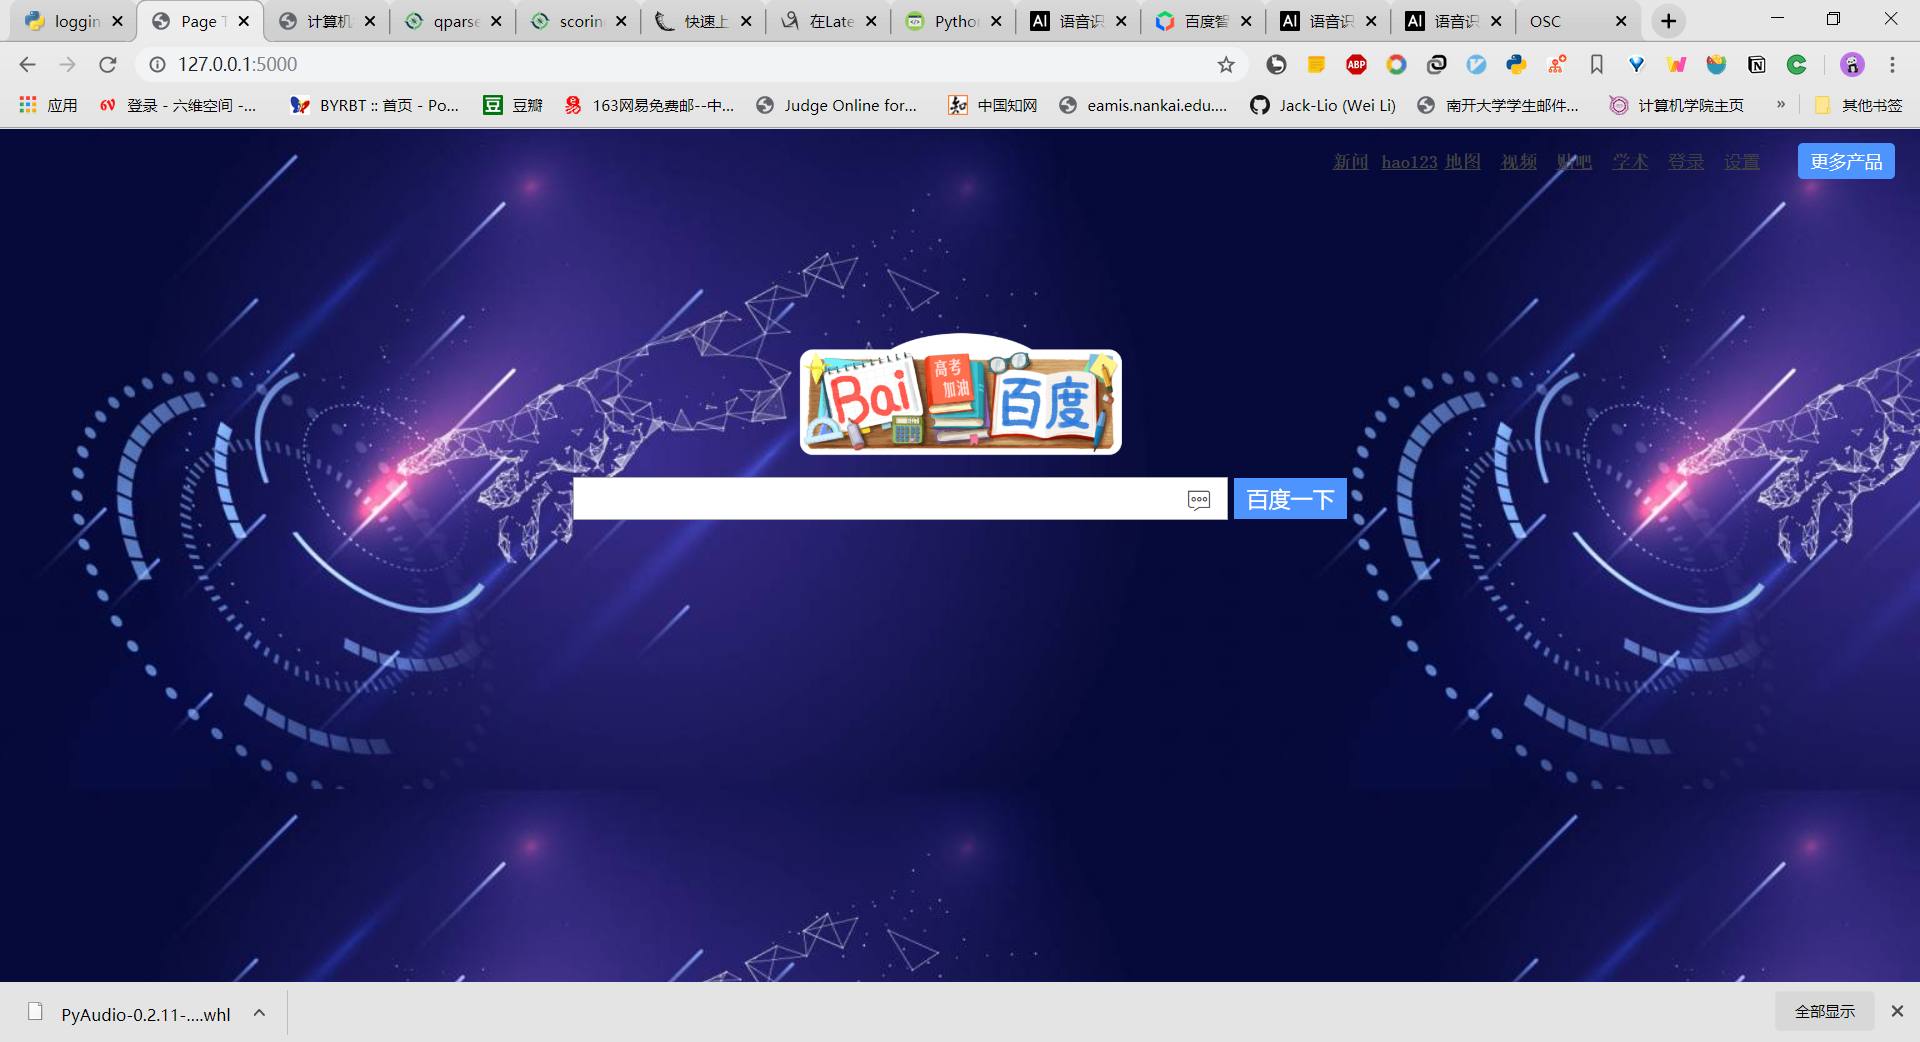
\includegraphics[width=0.6\textwidth]{2}
	\caption{教师信息搜索系统截图1——主页 \label{fig:2}}
\end{figure}

\begin{figure}[htbp]
	\centering
	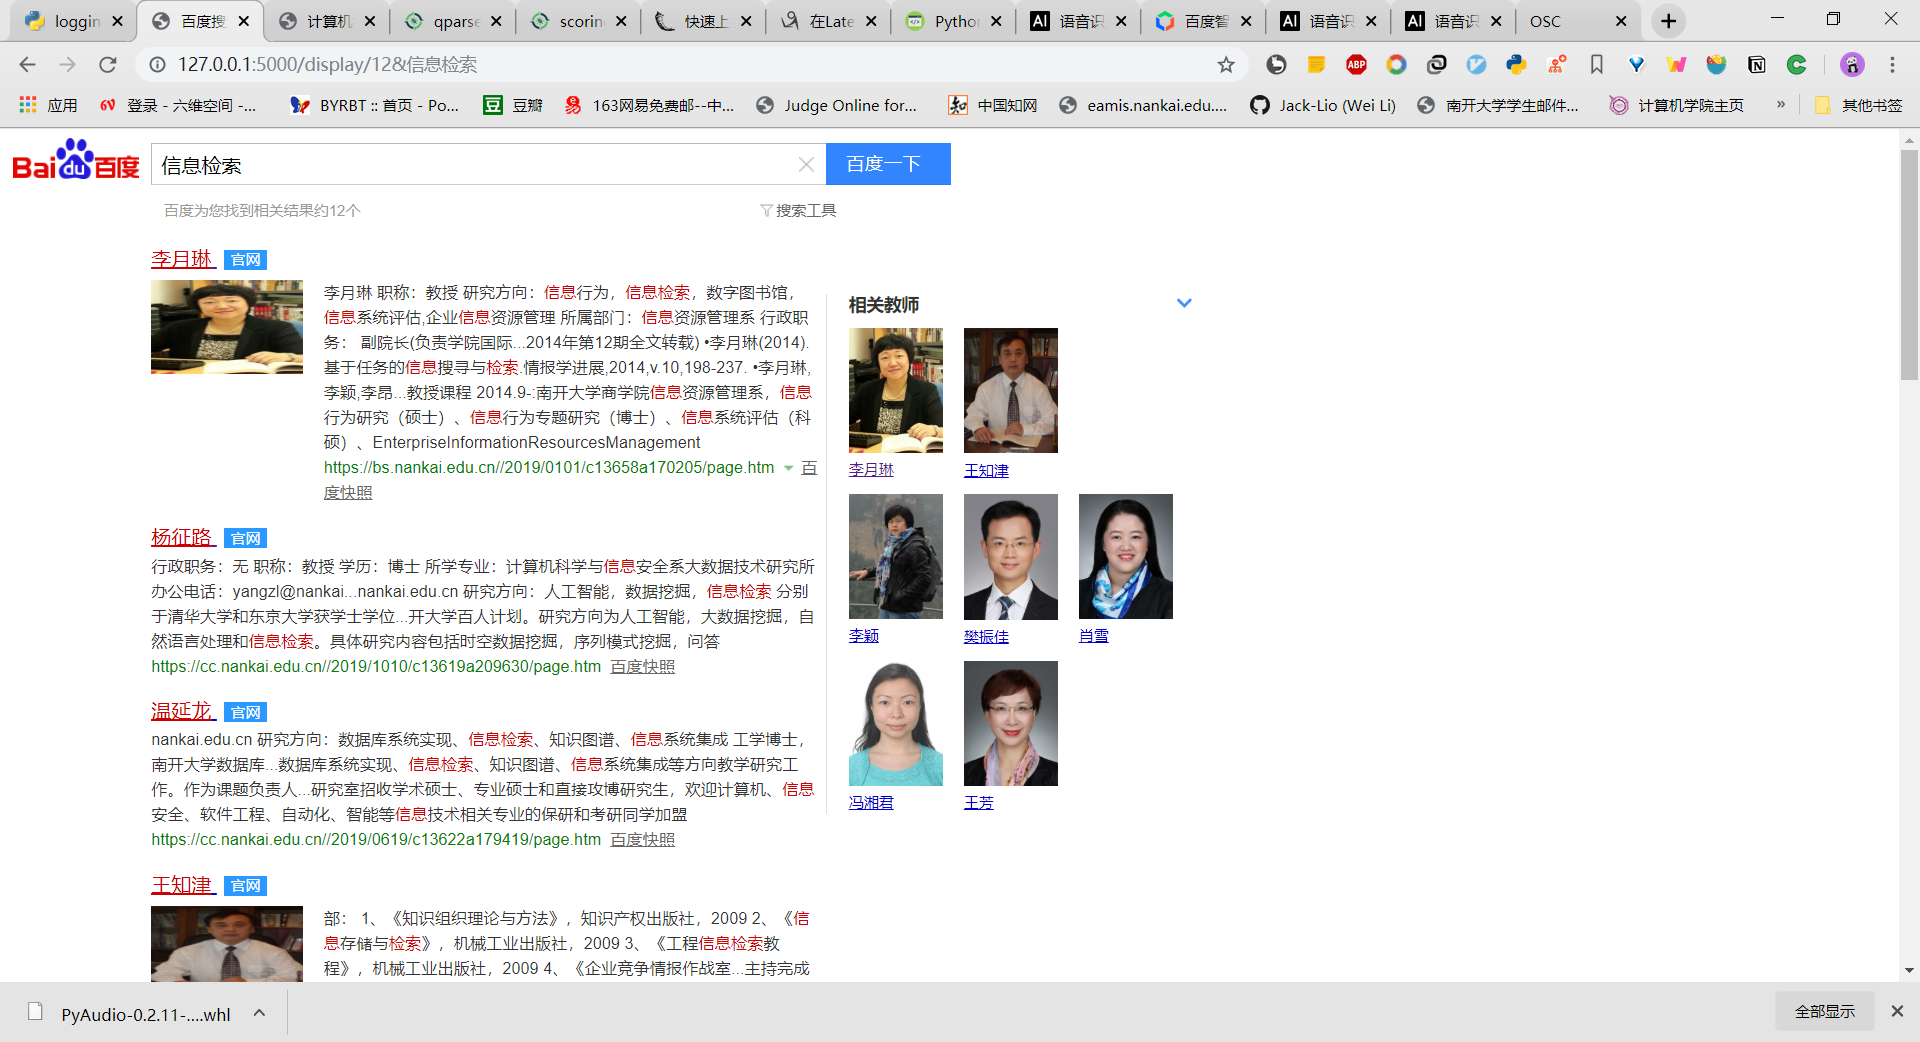
\includegraphics[width=0.6\textwidth]{3}
	\caption{教师信息搜索系统截图2——结果显示 \label{fig:3}}
\end{figure}

查询界面的实现借用了百度的相关样式文件,在其基础上进行修改后得到,具体实现将在后续的实现步骤中说明。

\section{实验具体步骤}

从实验分析和实验思路上可以了解到,本次实验主要分为三个步骤实现,分别是数据爬取,索引构建,查询服务实现,以下主要从这三个方面结合代码介绍本次实验的具体实现步骤,怎样从数据获取一直到得到功能完备的web搜索系统。

\subsection{数据爬取实现}

数据爬取基于scrapy爬虫框架实现,由于这个框架构建了完备的缓冲机制和多线程机制,所以能够实现很快的爬虫功能。其次通过框架实现能够避免很多的重复工作。由于对不同网站的爬虫代码只有微笑的差异,所以接下来将主要基于对计算机学院的爬虫代码进行解析说明:

\begin{lstlisting}[language =Python, numbers=left, 
numberstyle=\tiny,keywordstyle=\color{blue!70},
commentstyle=\color{red!50!green!50!blue!50},frame=shadowbox,
rulesepcolor=\color{red!20!green!20!blue!20},basicstyle=\ttfamily]

		##############################
		# spider for cs
		# filename:spider_cc.py
		# author:  liwei
		# StuID:   1711350
		# date:    2019.12.1
		##############################
		import scrapy
		import os
		snapshots_path = '../query_system/templates/snapshots'          # 网页快照保存位置
		
		class CCTeacherInfoSpider(scrapy.Spider):
		name = "cc"
		# 创建存储爬取信息的文件夹
		if not os.path.exists('../docs/%s'%name):
		os.mkdir('../docs/%s'%name)
		
		if not os.path.exists('../docs/%s/m_text' % name):      # 锚文本存储文件夹
		os.mkdir('../docs/%s/m_text' % name)
		
		if not os.path.exists('%s/%s' % (snapshots_path,name)):      # 网页快照存储文件夹
		os.mkdir('%s/%s' % (snapshots_path,name))
		# if os.path.exists('../docs/%s/index.txt'%name):
		#     os.remove('../docs/%s/index.txt'%name)
		
		baseurl = 'https://cc.nankai.edu.cn/'
		def start_requests(self):
		urls = [
		'https://cc.nankai.edu.cn/jswyjy/list.htm',
		'https://cc.nankai.edu.cn/fjswfyjy/list.htm',
		'https://cc.nankai.edu.cn/js/list.htm',
		'https://cc.nankai.edu.cn/syjxdw/list.htm',
		
		]
		for url in urls:
		yield scrapy.Request(url=url, callback=self.parse)
		
		def parse(self, response):
		# 得到锚文本
		teacherItems = response.xpath('//table[@class="table table-striped table-bordered"]')
		# 获取每位老师具体介绍页面链接锚文本
		nexturls = teacherItems.css('a')
		# 输出链接数据
		file = open('../docs/%s/index.txt'%self.name,'a',encoding='utf-8')
		for urlt in nexturls:
		file.write(urlt.xpath('text()').get()+","+self.baseurl+urlt.xpath("@href").get()+","+"南开大学计算机学院"+","+response.url+'\n')
		# 保存锚文本
		m_f = open('../docs/%s/m_text/%s_m.txt' % (self.name, urlt.xpath('text()').get()), 'w', encoding='utf-8')
		m_f.write(str(urlt.get()))
		m_f.close()
		# 递归回调解析教师信息的解析器
		yield scrapy.Request(url=self.baseurl+urlt.xpath("@href").get(), callback=self.parseTeacher)
		file.close()
		
		
		def parseTeacher(self,response):
		details = response.xpath('//div[@class="body-introduce"]')
		
		filename = str(details.xpath('.//div[@class="form col-md-7"]/p[1]/span[2]/text()').get()).replace('\n','').replace(' ','').replace('\r','')
		
		# 保存网页快照
		with open('%s/%s/%s.html' % (snapshots_path, self.name, filename), 'wb')as s_f:
		s_f.write(response.body)
		f = open('../docs/%s/%s.txt'%(self.name,filename),'w',encoding='utf-8')
		for item in details.xpath('.//div[@class="form col-md-7"]').css("p"):
		if item.css("span").get() is  None:
		if item.xpath("text()").get() is not None:
		f.write(item.xpath("text()").get()+'\n')
		else:
		if item.xpath('./span[@class = "attribute"]/text()').get() is  not None  and item.xpath('./span[2]/text()').get()is  not None :
		f.write(str(item.xpath('./span[@class = "attribute"]/text()').get()+item.xpath('./span[2]/text()').get()).replace('\n','').replace(' ','').replace('\r','')+"\n")
		for item in details.xpath('.//div[@id="PersonalProfile"]//p'):
		if item.get() is not  None:
		for text in item.xpath('.//text()').getall():
		f.write(text)
		f.write('\n')
		f.close()
\end{lstlisting}

从上述代码中可以看到,首先通过引入scrapy工具包,创建存储数据的文件路径,通过request请求获取几个baseurl指向网页,通过解析网页的源码结构,利用xpath解析路径,定位锚文本,获取教师主页的链接进一步采用request请求获取HTML代码,从而进一步解析数据进行存储,将获取的数据存储到指定的文件路径中去。

\begin{figure}[htbp]
	\centering
	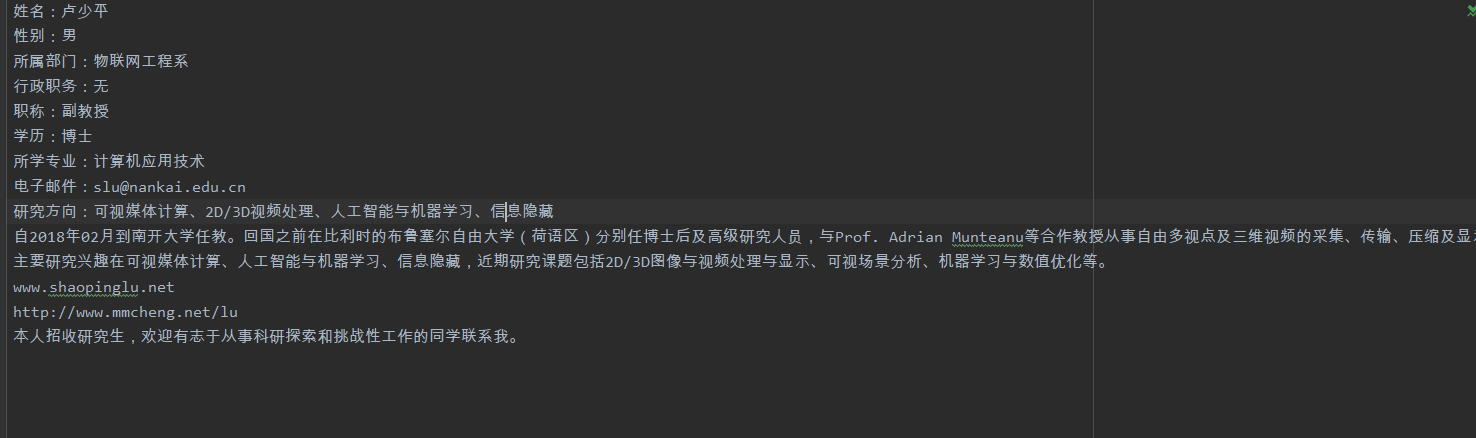
\includegraphics[width=0.6\textwidth]{4}
	\caption{爬取的教师信息样例 \label{fig:4}}
\end{figure}

\subsection{索引构建实现}

索引的构建基于实验思路中建立的索引对象的field设置,通过将响应的文本填入对应的field中,whoosh能够自动的构建索引并且将索引数据存储到制定的文件路径下供后续使用。

构建索引的主要代码如下所示:

\begin{lstlisting}[language = Python, numbers=left, 
numberstyle=\tiny,keywordstyle=\color{blue!70},
commentstyle=\color{red!50!green!50!blue!50},frame=shadowbox,
rulesepcolor=\color{red!20!green!20!blue!20},basicstyle=\ttfamily]
# 构建索引目录
if not os.path.exists('index'):             #如果目录index不存在则创建
os.mkdir('index')
ix = index.create_in("index",schema)        #按照schema模式建立索引目录
ix = index.open_dir("index")                #打开该目录一遍存储索引文件

#索引构建,基于路径的基本索引
writer = ix.writer()
count = 0
# 遍历根目录对索引文本内容构建索引
for item in info.keys() :
path_ct = get_content(info[item]['xueyuan'],info[item]["name"])
path_mt = get_mtext(info[item]['xueyuan'],info[item]["name"])
path_ht = get_html(info[item]['xueyuan'],info[item]["name"])
path_img = get_img(info[item]['xueyuan'],info[item]["name"])
print("=======>" + path_ct,path_ht,path_img,path_mt)
# 获取信息文本
content = ''
if os.path.exists(path_ct):
f = open(path_ct, 'r', encoding='UTF-8')
for line in f:
content = content + line
f.close()
# 获取锚文本
m_text = ''
if os.path.exists(path_mt):
mf = open(path_mt, 'r', encoding='UTF-8')
for line in mf:
m_text = m_text + line
mf.close()

writer.add_document(title=info[item]['name'],
url=info[item]['url'],
content=content,
path=path_ct,
mtext=m_text,
xueyuan=info[item]['xueyuan'],
shotpath= path_ht,
picpath= path_img,
parenturl=info[item]['parentUrl'],
)
count = count + 1
writer.commit()
print("==========>共索引文件%d个"%count)
\end{lstlisting}



从代码中可以看到主要的步骤为两个,构建索引存储目录以及将索引文本传入索引构建器中。在写入索引文本之后,提交输入的索引文本,whoosh自动开始构建索引。


\subsection{查询服务实现}
查询界面的样式文件基于百度修改得到,基本贴近真实的浏览器功能,能够支持较为人性化的交互。查询功能的实现主要基于whoosh提供的接口,并融入了自定义的pagerank对网页的可信度进行评分,得到pagerank排序。

实现的查询服务主要包括前缀查询、短语查询、正则表达式查询、多域混合查询和按域查询等。实现的主要代码如下所示:

\begin{lstlisting}[language = Python, numbers=left, 
numberstyle=\tiny,keywordstyle=\color{blue!70},
commentstyle=\color{red!50!green!50!blue!50},frame=shadowbox,
rulesepcolor=\color{red!20!green!20!blue!20},basicstyle=\ttfamily]
	#查询构建
	from whoosh import highlight
	from whoosh import qparser
	from whoosh import index
	from flask import Flask
	from flask import request
	from flask import jsonify,render_template,abort, redirect, url_for,session, escape,Markup
	from flask_cors import  *
	import re
	import logging
	from numpy import std
	from data import xy_dict
	from data import get_html,get_teacher_info,pagerank
\end{lstlisting}

通过引入flask相关包实现后台的构建和网页路由和响应功能,引入whoosh的相关模块实现查询服务。

\begin{lstlisting}[language =Python, numbers=left, 
numberstyle=\tiny,keywordstyle=\color{blue!70},
commentstyle=\color{red!50!green!50!blue!50},frame=shadowbox,
rulesepcolor=\color{red!20!green!20!blue!20},basicstyle=\ttfamily]
	# from audio import *     # 未完全实现
	
	app = Flask(__name__)
	CORS(app,supports_credentials=True)    # 解决跨域请求无响应问题
	app.secret_key=b'\xfa\n\x08\xb9\x84I\xe5xRdE\xea\x9f\xba\xce\x81'
	mysession =dict()                      # 自定义的session用来传输数据
	url_dict,scores = pagerank(get_teacher_info())      # 获取pageranke计算结果,返回链接映射和排名得分
	# 定义日志记录文件的配置
	LOG_FORMAT = "%(asctime)s - %(levelname)s - %(message)s"
	DATE_FORMAT = "%m/%d/%Y %H:%M:%S %p"
	
	logging.basicConfig(filename='my.log', level=logging.DEBUG, format=LOG_FORMAT, datefmt=DATE_FORMAT)
	
	ix = index.open_dir("index")            #打开该目录一遍存储索引文件
\end{lstlisting}

在定义区定义了包括后台服务对象APP,自定义数据传送单元mysession,索引对象目录等在内的诸多全局参数。


\begin{lstlisting}[language =Python, numbers=left, 
numberstyle=\tiny,keywordstyle=\color{blue!70},
commentstyle=\color{red!50!green!50!blue!50},frame=shadowbox,
rulesepcolor=\color{red!20!green!20!blue!20},basicstyle=\ttfamily]
	
	# 基本查询函数,实现前缀、通配、正则匹配,短语、关系运算查询功能
	# 基于whoosh的highlighter实现返回高亮查询词块
	@app.route('/index',methods=['GET','POST'])
	def base_query():
	assert request.path == '/index'
	#print(dict(request.form)["query"][0])
	#print(dict(request.form))
	query_sentence = str(dict(request.form)["query"][0])
	logging.info("Query sentence: %s"%query_sentence)
	res = []
	with ix.searcher() as searcher:
	# 对输入的查询文本进行解析,如果存在按域查询的需求则区分按域查询,默认采用多属性查询模式
	# mark 表示是否需要高亮学院查询区域,默认情况下需要
	highlight_xy = True
	# 默认的多域查询
	query = qparser.MultifieldParser(["content","title","mtext","xueyuan"], ix.schema)
	if query_sentence.endswith("$姓名$"):
	# 按名字查询
	query =qparser.SimpleParser("title",ix.schema)
	query_sentence=query_sentence.strip('$姓名$')
	elif query_sentence.endswith("$学院$"):
	# 按学院查询
	query = qparser.SimpleParser("xueyuan", ix.schema)
	query_sentence=query_sentence.strip('$学院$')
	
	elif query_sentence.endswith("$网页$"):
	# 按网页内容查询
	query = qparser.SimpleParser("content", ix.schema)
	query_sentence=query_sentence.strip('$网页$')
	
	#print(query_sentence)
	# 引入查询解析器插件
	query.add_plugin(qparser.WildcardPlugin)
	
	# query.remove_plugin_class(qparser.WildcardPlugin)
	query.add_plugin(qparser.PrefixPlugin())
	query.add_plugin(qparser.OperatorsPlugin)
	query.add_plugin(qparser.RegexPlugin)
	query.add_plugin(qparser.PhrasePlugin)
	
	# 解析得到查询器
	q = query.parse(query_sentence)
	logging.info("Query parse result: %s"%str(q))
	print(q)
	# 获取查询结果
	result = searcher.search(q,limit=20)
	# print(result)
	# 设置碎片的属性
	# Allow larger fragments
	my_cf = highlight.ContextFragmenter(maxchars=200, surround=30)
	hf = highlight.HtmlFormatter( tagname='em', classname='match', termclass='term')
	
	hi = highlight.Highlighter(fragmenter=my_cf,formatter=hf)
	for hit in result:
	print(hit["picpath"])
	print(hit["title"])
	print(escape(hi.highlight_hit(hit,"content")))
	if hit['picpath'] =='#':
	if highlight_xy:
	res.append({"title": hit['title'],
		"xueyuan": Markup(hi.highlight_hit(hit, "xueyuan")),
		"url": hit["url"],
		'shotpath': hit['shotpath'],
		"content": Markup(hi.highlight_hit(hit, "content")),
		"parenturl": hit["parenturl"],
		"picpath": '#',
		"pagerank":scores[url_dict[hit["url"]]]
	})
	else:
	res.append({"title": hit['title'],
		"xueyuan": hit["xueyuan"],
		"url": hit["url"],
		'shotpath': hit['shotpath'],
		"content": Markup(hi.highlight_hit(hit, "content")),
		"parenturl": hit["parenturl"],
		"picpath": '#',
		"pagerank":scores[url_dict[hit["url"]]]
	})
	else:
	if highlight_xy:
	res.append({"title":hit['title'],
		"xueyuan":Markup(hi.highlight_hit(hit, "xueyuan")),
		"url":hit["url"],
		'shotpath':hit['shotpath'],
		"content":Markup(hi.highlight_hit(hit,"content")),
		"parenturl": hit["parenturl"],
		"picpath":"images/%s/%s"%(hit['picpath'].split('/')[-3],hit['picpath'].split('/')[-1]),
		"pagerank": scores[url_dict[hit["url"]]]
	})
	else:
	res.append({"title": hit['title'],
		"xueyuan": hit["xueyuan"],
		"url": hit["url"],
		'shotpath': hit['shotpath'],
		"content": Markup(hi.highlight_hit(hit, "content")),
		"parenturl": hit["parenturl"],
		"picpath": "images/%s/%s" % (
		hit['picpath'].split('/')[-3], hit['picpath'].split('/')[-1]),
		"pagerank": scores[url_dict[hit["url"]]]
	})
	print(len(result))
	print(res)
	count = len(result)
	
	if count ==0:
	logging.warning("%d,没有查询到相关内容!"%404)
	return "没有查询到相关内容!",404
	else:
	# 记录查询日志
	log = "Response: "
	for item in res:
	log = log + " (name:%s,url:%s) " % (item["title"], item["url"])
	logging.info(log)
	
	# 基于page rank 对链接进行排序
	res.sort(key=lambda k:(k.get("pagerank",0)),reverse = True)
	print(res)
	
	mysession["data"] = res                       # 使用会话session传递参数
	return  jsonify({"url":"/display/%d&%s"%(count,query_sentence)})
		
\end{lstlisting}

从代码中可以看到,通过解析查询文本判断是否为特定形式的按域选择查询的查询方式,并进行解析,选择不同的查询模式,之后通过add\_plugi的方式添加支持不同查询功能的查询插件,能够提供不同的查询支持,最后通过将解析后的查询文本传入whoosh提供的seacher查询器中进行查询,将查询的结果形成json格式数据,并联合pagerank进行链接排序,将查询的结果返回给前端请求,为了简化查询的复杂度同时减轻前端压力,在此次实验中只返回了前20个查询结果。

\subsection{链接分析}

为了进行链接分析,需要获取网页地址之间的指向关系,在爬取数据的时候需要考虑这一点,将网页之间的父子对应关系也要存储下来,在我实现的系统中,保存这种关系是在数据爬取中进行的,数据截图如\figref{fig:5}所示:

\begin{figure}[htbp]
	\centering
	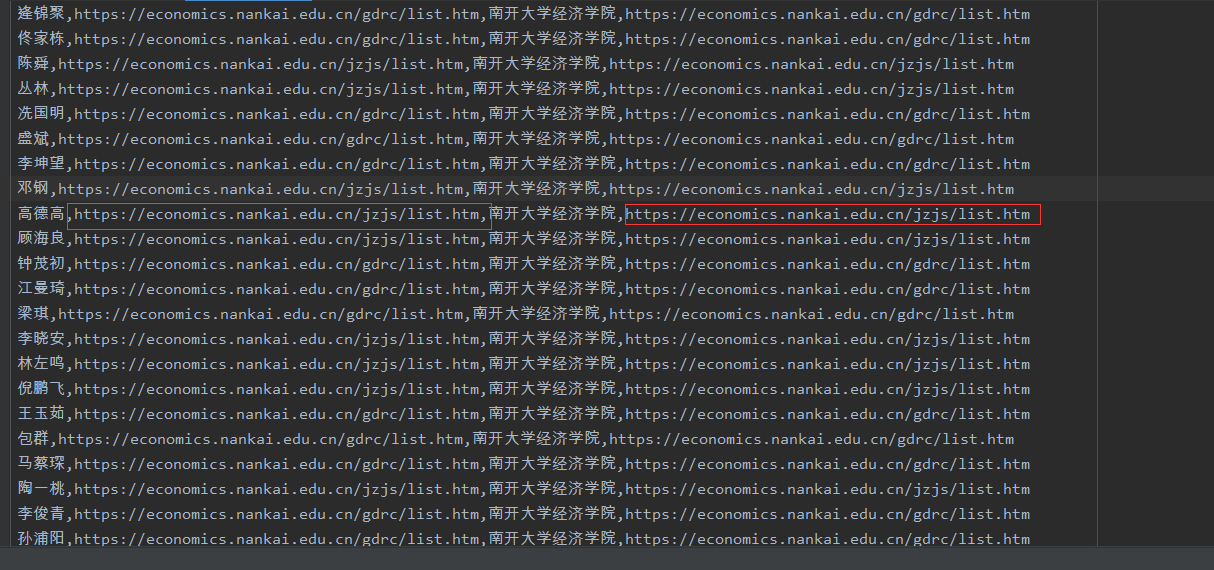
\includegraphics[width=0.6\textwidth]{5}
	\caption{爬取的链接关系数据截图 \label{fig:5}}
\end{figure}

通过解析这种链接关系可以构建马尔科夫随机游走概率矩阵,通过多重迭代,实现最后稳定的pagerank分值就是所要求的的结果,这部分工作在数据处理单元data.py文件中实现,函数代码如下所示:

\begin{lstlisting}[language = Python, numbers=left, 
numberstyle=\tiny,keywordstyle=\color{blue!70},
commentstyle=\color{red!50!green!50!blue!50},frame=shadowbox,
rulesepcolor=\color{red!20!green!20!blue!20},basicstyle=\ttfamily]
	
	# 根据爬取的静态网页链接分析获取pagerank的值,info为获取的所有教师数据,info字段如下
	# "name": item_list[0],
	# "url": item_list[1],
	# "xueyuan": item_list[2],
	# "parentUrl": item_list[3],
	# "pageRefer": 1,
	def pagerank(info_t):
	info = dict(info_t)
	url_dict = dict()   # 存储网页编号映射关系
	url_pair = {}       # 存储网页指向对
	no = 0
	# 形成所有网页的序号映射表
	for key in info.keys():
	if info[key]["url"] not in url_dict.keys():
	url_dict[info[key]["url"]] = no
	no = no + 1
	if info[key]["parentUrl"] not in url_dict.keys():
	url_dict[info[key]["parentUrl"]] = no
	no = no + 1
	if info[key]["parentUrl"] not in url_pair.keys():
	url_pair[info[key]["parentUrl"]] = [info[key]["url"]]
	else:
	url_pair[info[key]["parentUrl"]].extend([info[key]["url"]])
	
\end{lstlisting}

通过解析保存的映射关系文本,获取连接对应关系,并对链接进行编号,方便构建矩阵。

\begin{lstlisting}[language = Python, numbers=left, 
numberstyle=\tiny,keywordstyle=\color{blue!70},
commentstyle=\color{red!50!green!50!blue!50},frame=shadowbox,
rulesepcolor=\color{red!20!green!20!blue!20},basicstyle=\ttfamily]
	# 形成随机游走过程概率矩阵
	N = len(url_dict.keys())        # 矩阵规模
	matrix = np.zeros((N,N))        # 声明矩阵
	# 计算邻接矩阵
	for parenturl in url_pair.keys():
	for sonurl in url_pair[parenturl]:
	matrix[url_dict[parenturl]][url_dict[sonurl]] = 1
	matrix[url_dict[sonurl]][url_dict[parenturl]] = 0
	# 马尔科夫链 转移矩阵
	for i in range(N):
	count = 0
	for j in range(N):               # 统计1 的数量
	if matrix[i][j] ==1 :
	count=count +1
	if count == 0 :               # 一行中没有1 ,全部置位1/N
	for j in range(N):
	matrix[i][j] = 1.0/N
	else:
	for j in range(N):
	if matrix[i][j]==1:         # 非全0 替换为1/count
	matrix[i][j]= 1.0/count
	alpha  =  0.1
	matrix1 = matrix*(1-alpha)
	matrix2 = matrix1+(alpha/N)
\end{lstlisting}

通过构建邻接矩阵进一步构建马尔科夫随机概率矩阵,用于后续的迭代过程。

\begin{lstlisting}[language = Python, numbers=left, 
numberstyle=\tiny,keywordstyle=\color{blue!70},
commentstyle=\color{red!50!green!50!blue!50},frame=shadowbox,
rulesepcolor=\color{red!20!green!20!blue!20},basicstyle=\ttfamily]
	# 设定初始的状态概率分布向量
	start = np.zeros((N,N))
	start[0][0] = 1
	cur = next = np.dot(start,matrix2)
	times = 0
	while(1):
	times =times+1
	exit_flag = True
	next = np.dot(cur,matrix2)     # 迭代
	
	for i in range(N):
	if next[0][i] != cur[0][i] :
	exit_flag = False
	if(exit_flag):
	break
	cur = next
	scores = next[0]
	print("end")
	return url_dict,scores              # 返回映射关系和page得分
\end{lstlisting}

通过设定一个初始的状态序列,经过不断的迭代知道稳定下来,稳定的向量数据就是pagerank所需要的分值,返回建立的链接编号数据以及计算得到的pagerank数据。

\section{结果展示}


\subsection{界面展示与功能说明}

\begin{figure}[htbp]
	\centering
	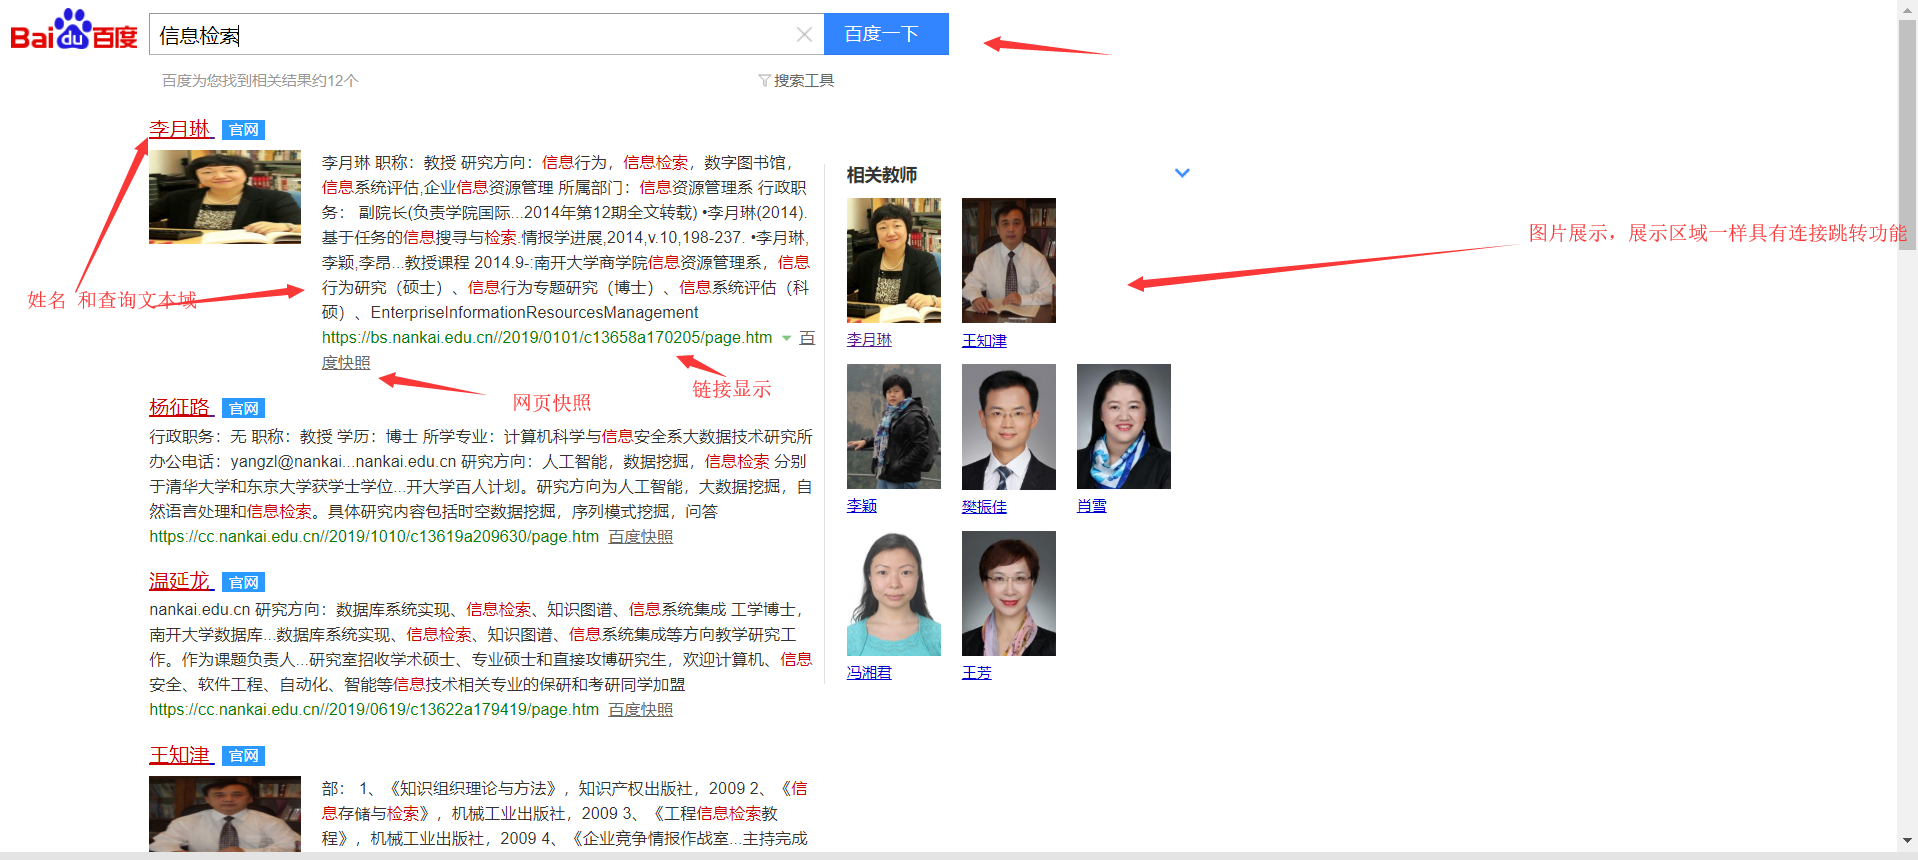
\includegraphics[width=0.6\textwidth]{6}
	\caption{查询结果界面展示与说明 \label{fig:6}}
\end{figure}

\subsection{短语查询}

\begin{figure}[htbp]
	\centering
	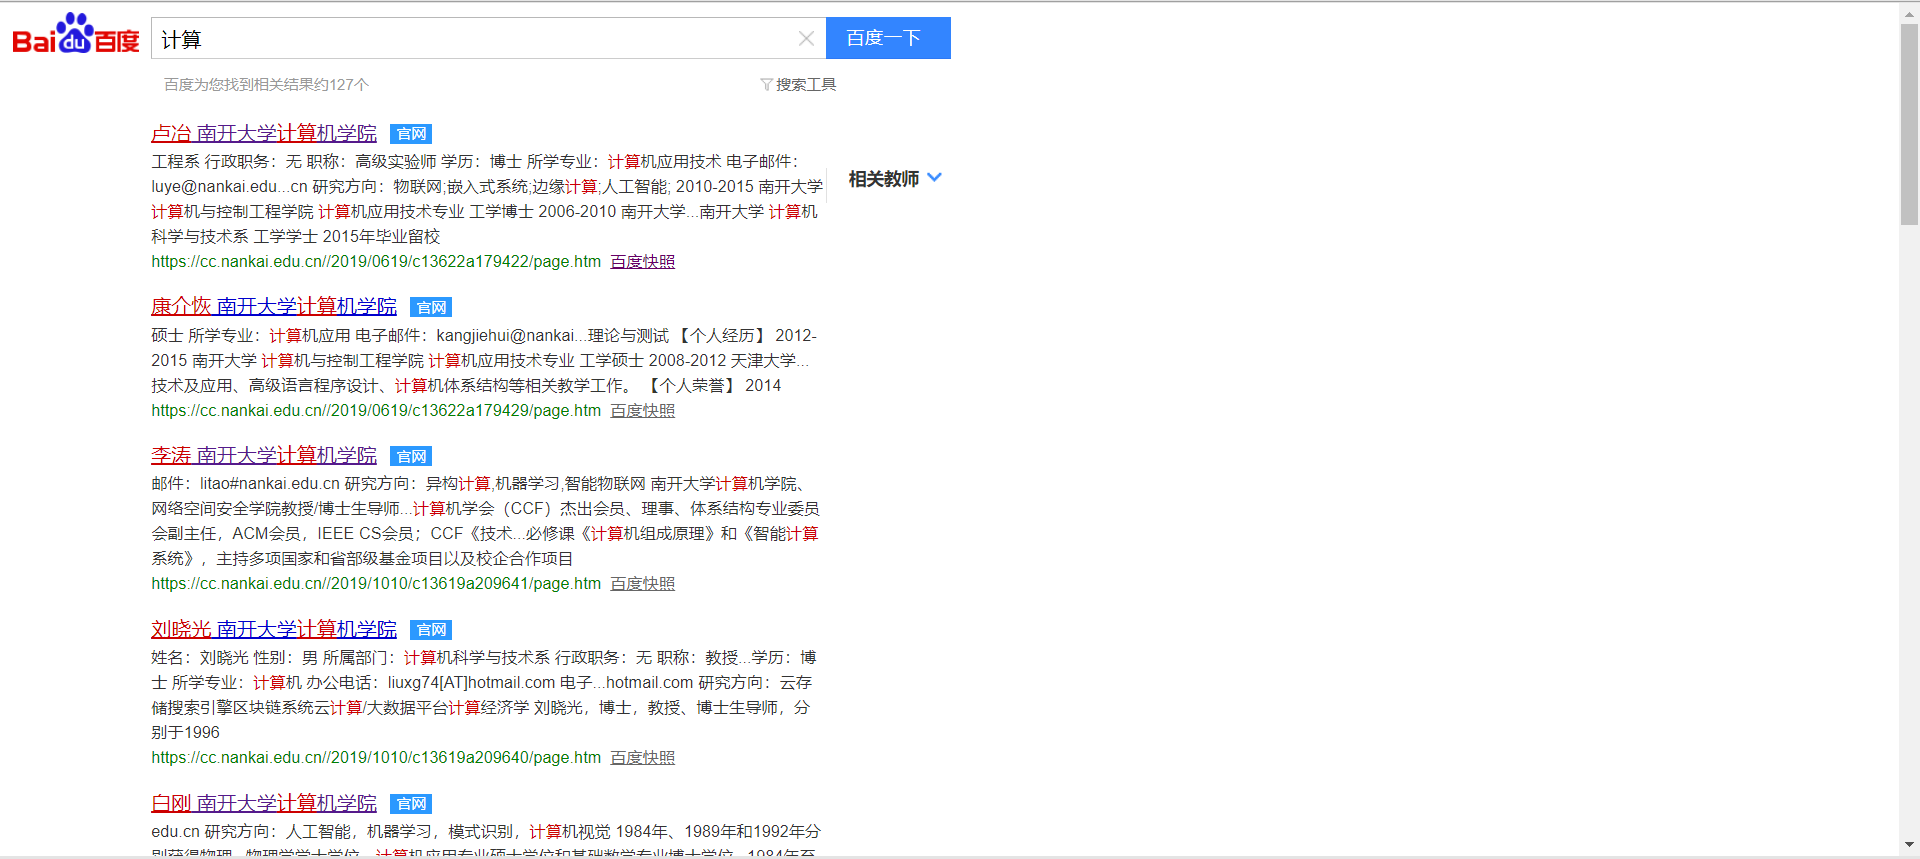
\includegraphics[width=0.6\textwidth]{14}
	\caption{短语查询 \label{fig:7}}
\end{figure}

\subsection{正则表达式查询}

\begin{figure}[htbp]
	\centering
	
\includegraphics[width=0.6\textwidth]{15}
	\caption{正则表达式查询 \label{fig:8}}
\end{figure}

\subsection{关系表达式查询}

\begin{figure}[htbp]
	\centering
	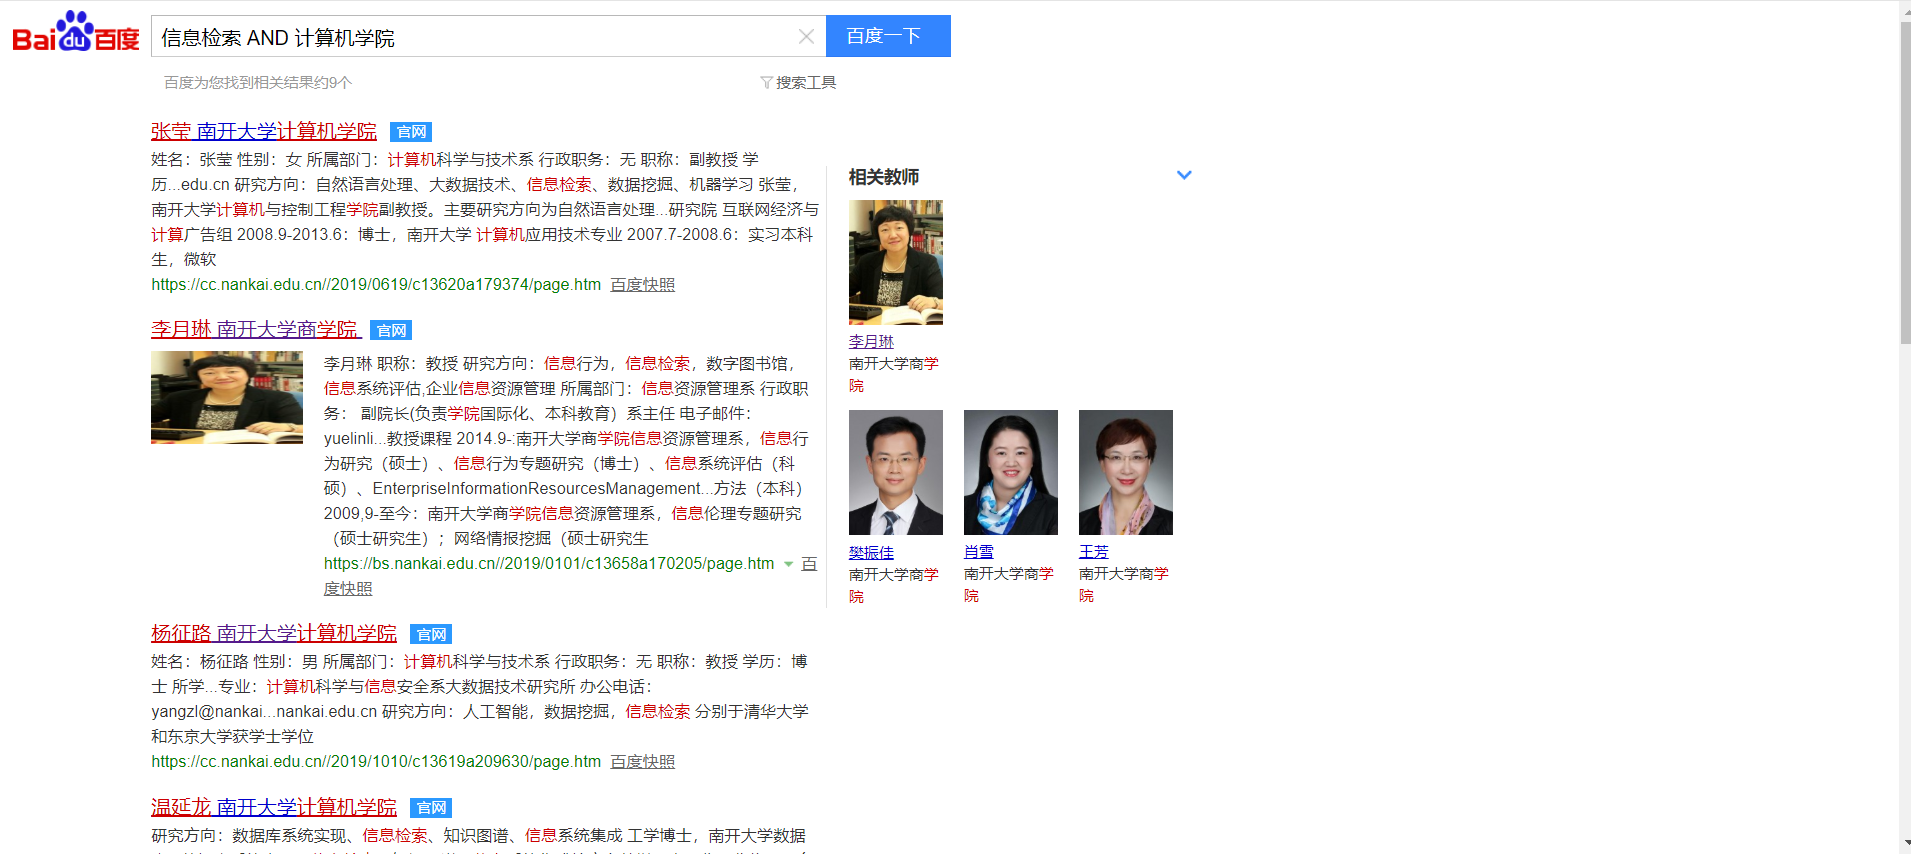
\includegraphics[width=0.6\textwidth]{7}
	\caption{关系表达式查询 \label{fig:9}}
\end{figure}

\subsection{混合查询和按域查询以及前缀查询}

\begin{figure}[htbp]
	\centering
	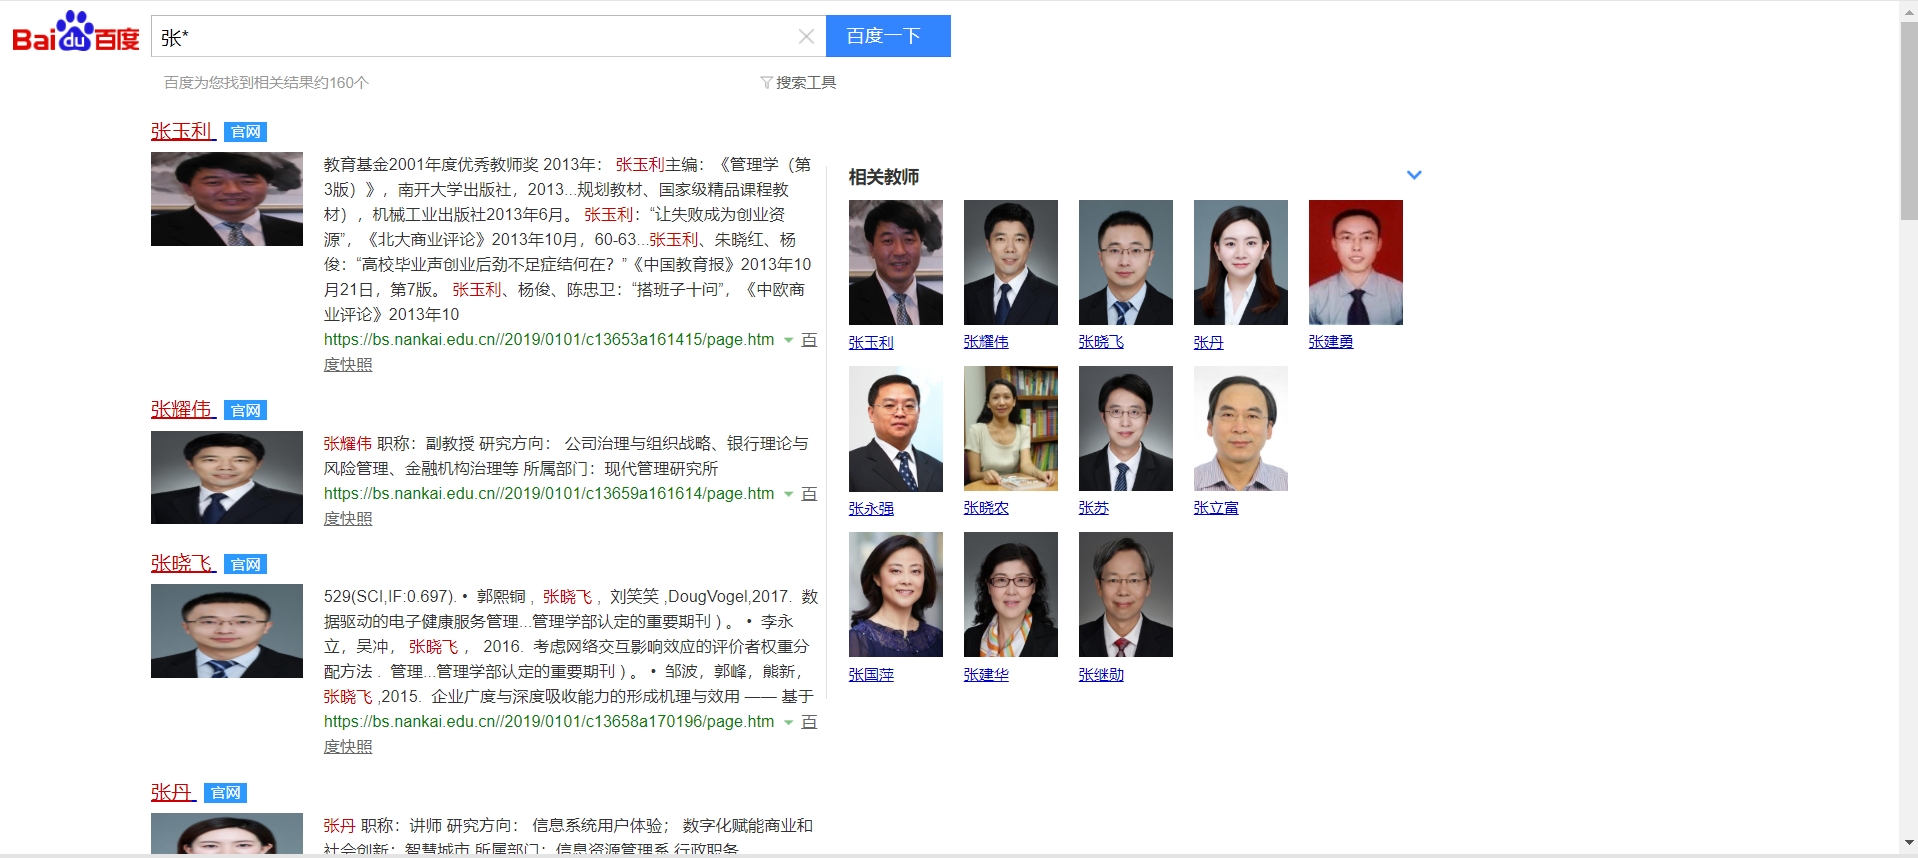
\includegraphics[width=0.6\textwidth]{8}
	\caption{混合查询与前缀查询\label{fig:10}}
\end{figure}

\begin{figure}[htbp]
	\centering
	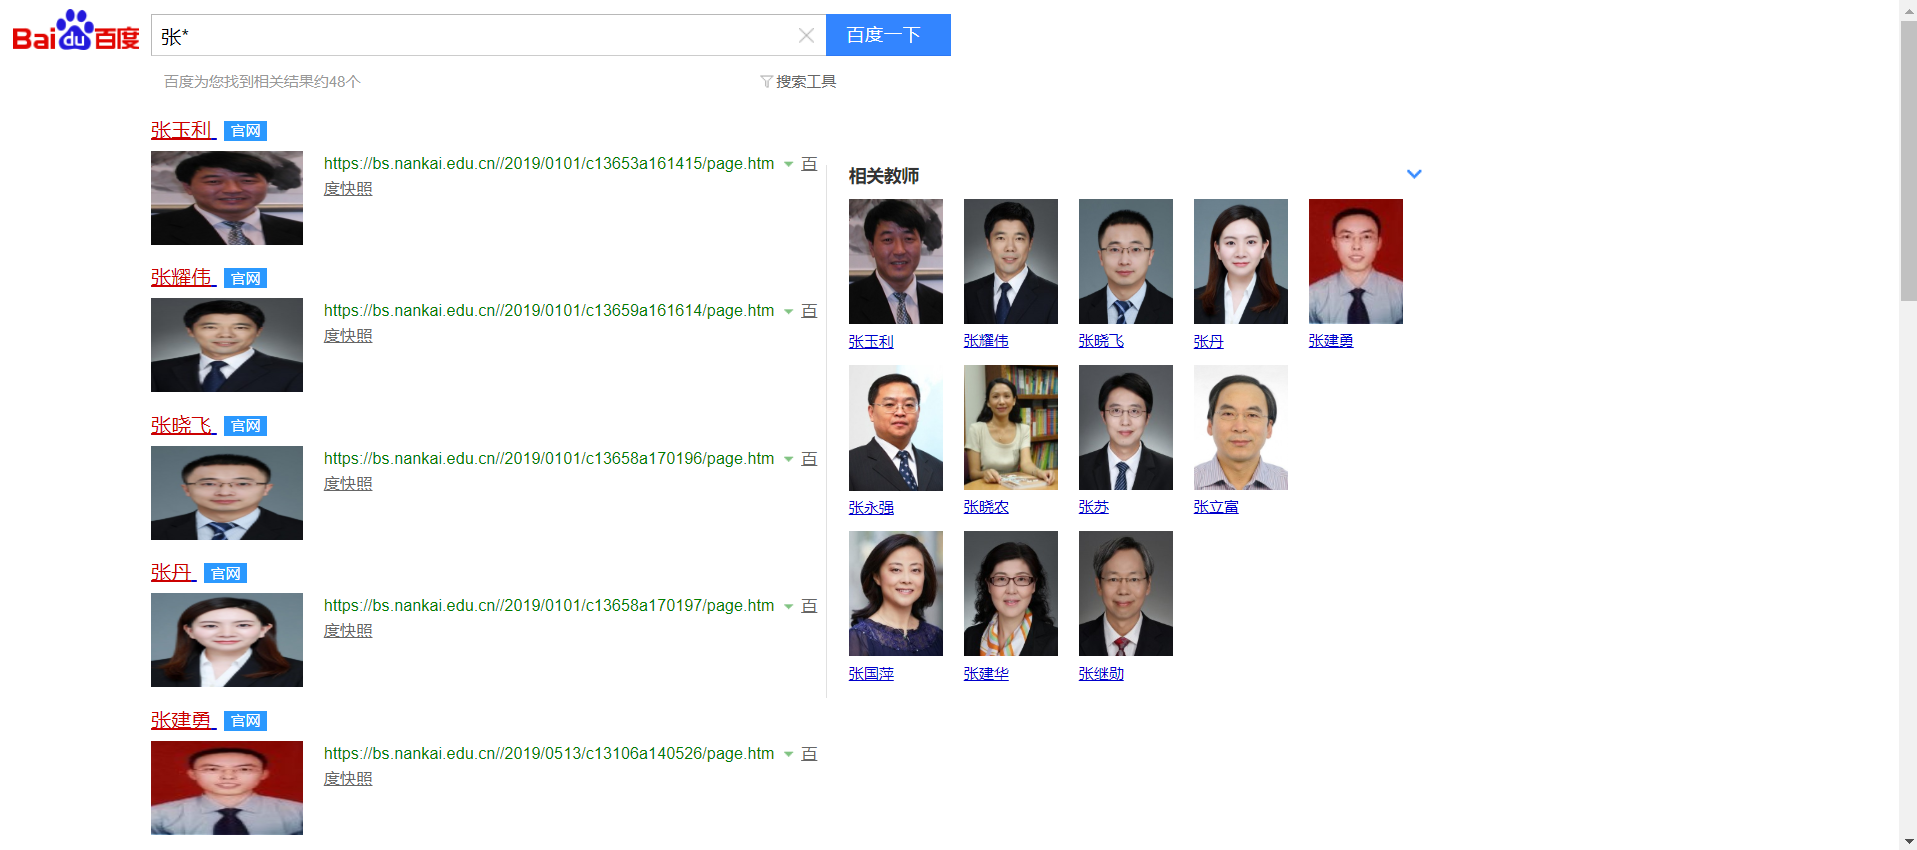
\includegraphics[width=0.6\textwidth]{9}
	\caption{按域查询\label{fig:13}}
\end{figure}

\subsection{链接分析}

\begin{figure}[htbp]
	\centering
	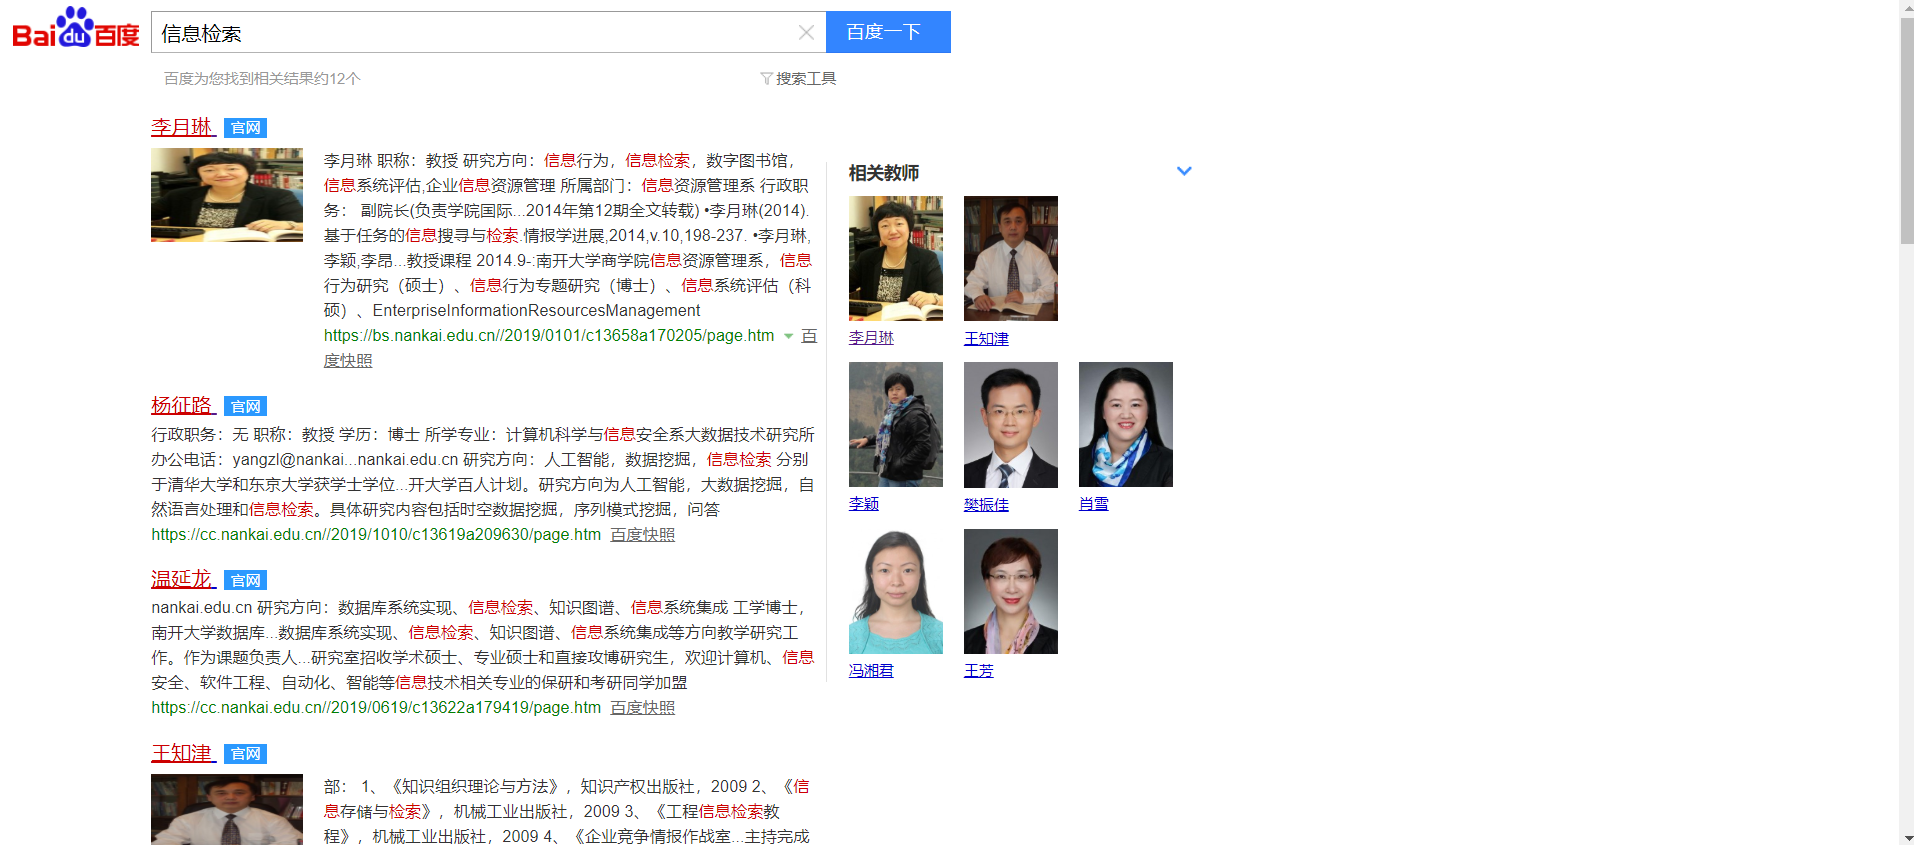
\includegraphics[width=0.6\textwidth]{12}
	\caption{无链接分析查询\label{fig:11}}
\end{figure}

\begin{figure}[htbp]
	\centering
	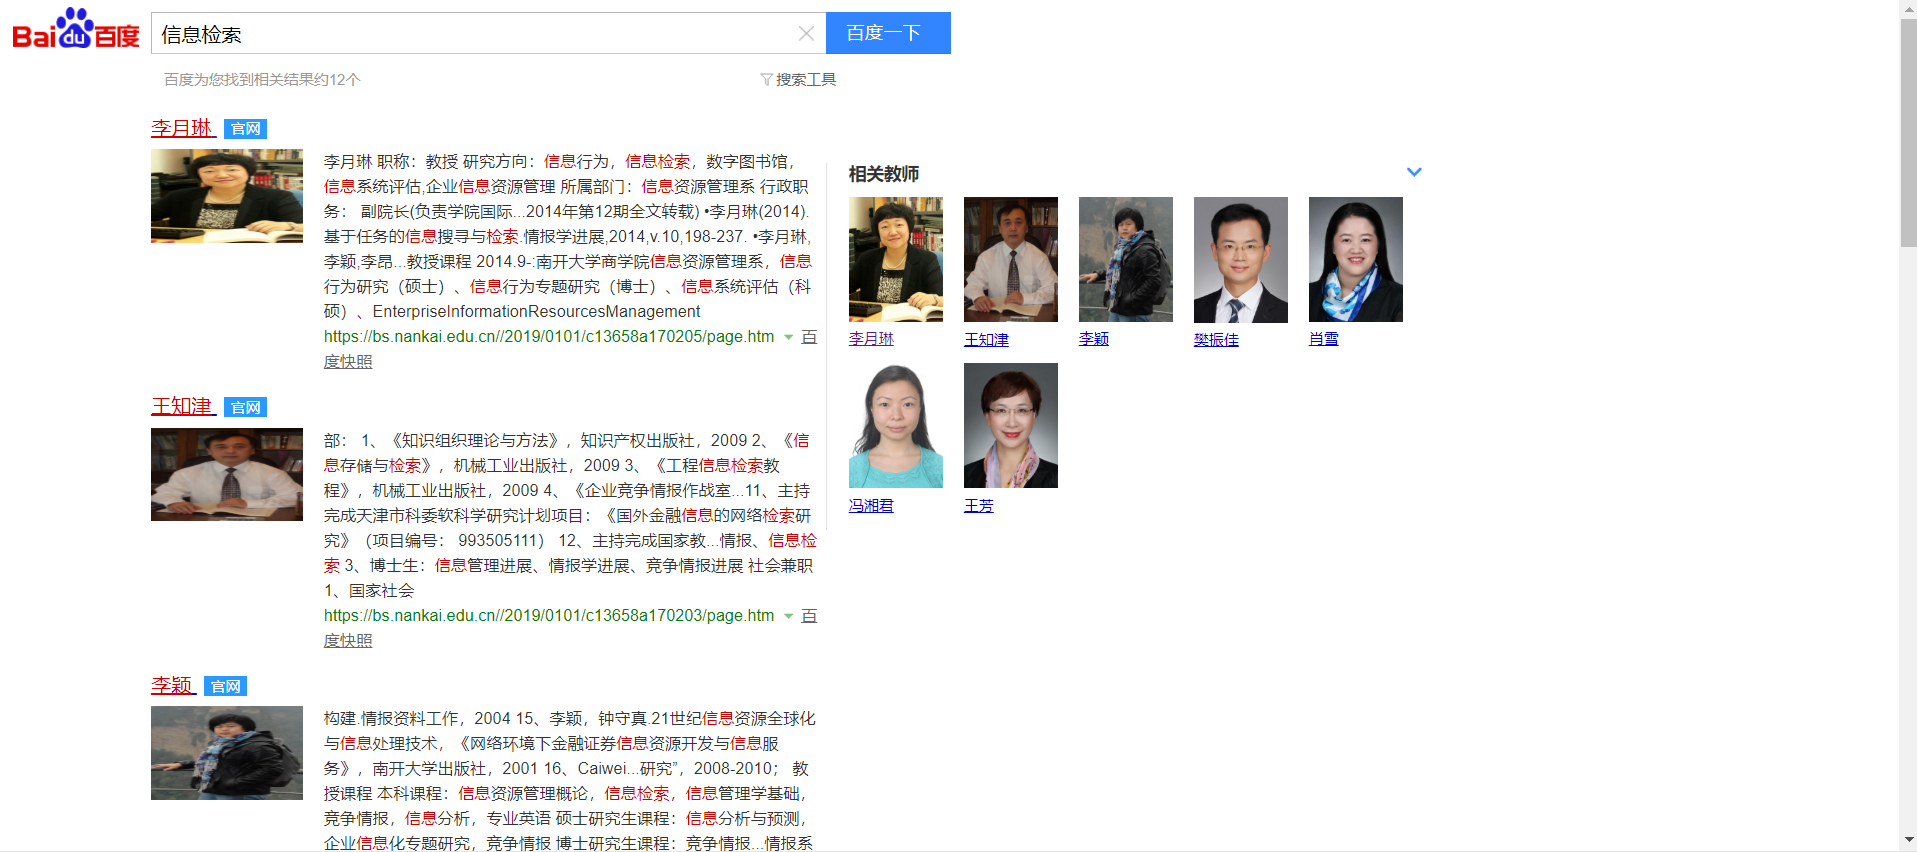
\includegraphics[width=0.6\textwidth]{13}
	\caption{加入链接分析模块查询 \label{fig:12}}
\end{figure}

\newpage
\section{总结与思考}
通过这次web搜索系統的构建实验,进一步将课堂上所学习的知识转化为实际的实践作业,更加加深了对于相关知识的理解,同时在这一次的实验中设计了大量的前端知识和相关工具包的使用,进一步锻炼了我的编程能力,虽然花了很长时间,但是最终昨晚感觉还是很有成就感的,在实现pagerank的过程中进一步理解了pagerank的计算和使用相关的知识,做到了学以致用,最后做出来的成品自己觉得还是很满意的,老师所要求的的所有基本功能差不多都实现了,自己针对页面和相关的交互还做了改进,本来还想做语音输入,但是电脑装不上pyaudio的工具包,最好没有全部做完,还是有点遗憾的。

\section{latex源码截图}

\begin{figure}[htbp]
	\centering
	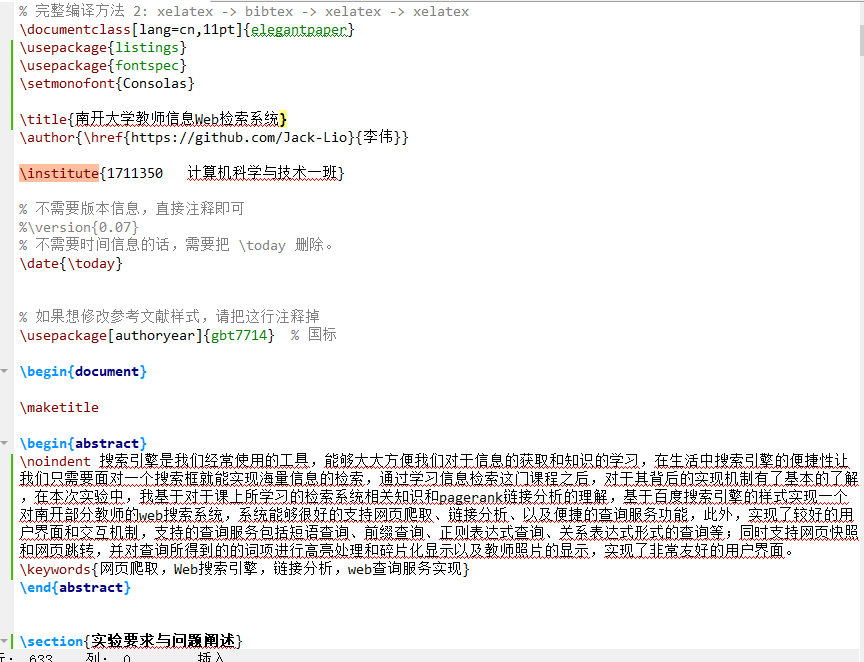
\includegraphics[width=0.6\textwidth]{16}
	\caption{源码1 \label{fig:15}}
\end{figure}

\begin{figure}[htbp]
	\centering
	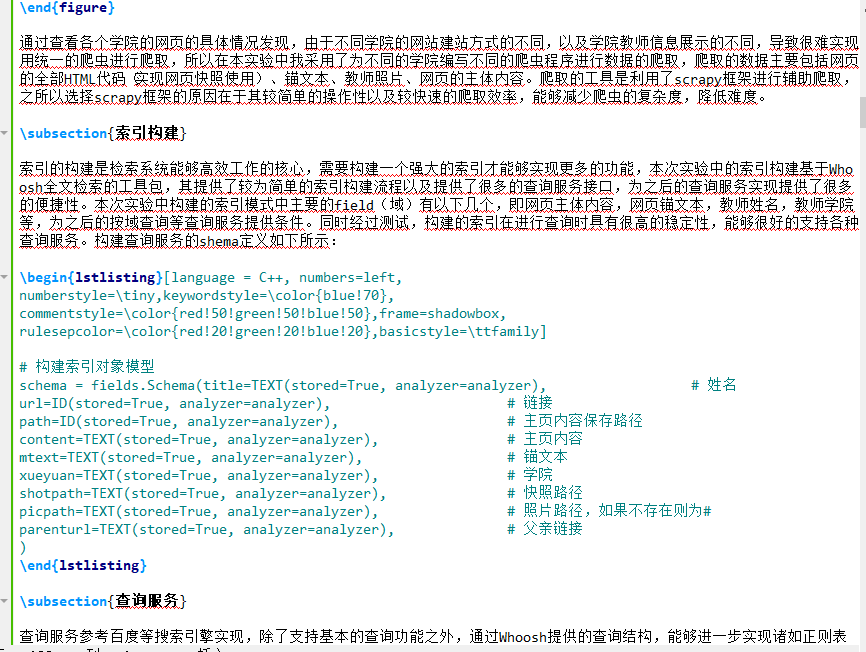
\includegraphics[width=0.6\textwidth]{17}
	\caption{源码2 \label{fig:16}}
\end{figure}

% 如果想修改参考文献样式(非国标),请把下行取消注释,并换成合适的样式(比如 unsrt,plain 样式)。
%\bibliographystyle{aer}
%\bibliography{wpref}

\end{document}
